\section{Dipolo eléctrico}

Se llama dipolo eléctrico a un sistema compuesto por dos cargas de igual magnitud y signo opuesto.

\begin{figure}[H]
    \centering
    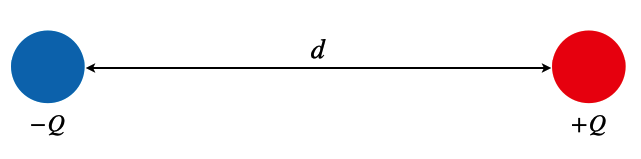
\includegraphics[width=0.59\textwidth]{Electroestática/Dipolos/dipolo.png}
\end{figure}

\subsection{Potencial}

En un sistema de referencia tal que las cargas están en el eje $z$ y el origen se ubica en el punto medio entre ambas el potencial del dipolo es

\begin{equation}
\begin{split}
    V(\Vec{r}) &= \frac{q}{4\pi\epsilon_o}\left(
    \frac{1}{\|\Vec{r}-d/2\hat{z}\|}-
    \frac{1}{\|\Vec{r}+d/2\hat{z}\|}\right)\\
     &= \frac{q}{4\pi\epsilon_o}\left(
    \frac{1}{\sqrt{x^2+y^2+(z-d/2)^2}}-
    \frac{1}{\sqrt{x^2+y^2+(z+d/2)^2}}\right)\\
\end{split}
\nonumber
\end{equation}
\bigbreak
\bigbreak
donde $d$ es la distancia entre las cargas. Si $x,y,z \gg d$ se puede aproximar $V$ por

\begin{equation}
\begin{split}
    V(\Vec{r}) &\approx \frac{q}{4\pi\epsilon_o}\left(
    \frac{1}{\sqrt{x^2+y^2+z^2-zd}}-
    \frac{1}{\sqrt{x^2+y^2+z^2+zd}}\right)\\
    &= \frac{q}{4\pi\epsilon_o}\left(
    \frac{1}{\sqrt{r^2-zd}}-
    \frac{1}{\sqrt{r^2+zd}}\right)\\
    &= \frac{q}{4\pi\epsilon_o r}\left(
    \frac{1}{\sqrt{1-zd/r^2}}-
    \frac{1}{\sqrt{1+zd/r^2}}\right)\\
    &\approx \frac{q}{4\pi\epsilon_o r}\left(
    1+\frac{zd}{2r^2}-\left(1-
    \frac{zd}{2r^2}\right)\right)\\
    &= \frac{qzd}{4\pi\epsilon_o r^3}
\end{split}
\nonumber
\end{equation}
\bigbreak
En coordenadas esféricas, $z=r\cos{\theta}$

\[V(\Vec{r})\approx\frac{qd\cos{\theta}}{4\pi\epsilon_o r^2}\]


\subsection{Momento dipolar}

Para un sistema de $n$ cargas, $\{q_i\}^n_{i=q}$, se define el momento dipolar como

\[\Vec{p}=\sum^n_{i=1}q_i\Vec{r_i}\]

En una distribución de carga continua se tiene

\[\Vec{p}=\int\Vec{r}\,dq(\Vec{r})\]
\bigbreak

El potencial eléctrico generado por un dipolo a \textbf{grandes distancia} es aproximado por

\[V(\Vec{r}) \approx \frac{1}{4\pi\epsilon_o}
\frac{1}{\|\Vec{r}-\Vec{r}'\|^3}\Vec{p}\cdot
(\Vec{r}-\Vec{r}')\]
\bigbreak

donde $\Vec{r}'$ es la posición del punto medio entre las cargas. Lo de grandes distancias es con respecto a $d$ la distancia entre las cargas del dipolo, es por eso que muchas veces se podrá usar esta expresión para puntos no muy alejados del dipolo.\\

El campo eléctrico a partir de este potencial está dado por

\[\Vec{E}= \frac{1}{4\pi\epsilon_o}
\frac{1}{\|\Vec{r}-\Vec{r}'\|^5}\left(3(\Vec{p}\cdot
(\Vec{r}-\Vec{r}'))(\Vec{r}-\Vec{r}')-\|\Vec{r}-\Vec{r}'\|^2\Vec{p}\,\right)\]
\bigbreak
El potencial eléctrico generado por una distribución de cargas arbitraria a grandes distancia se puede aproximar por

\[V(\Vec{r}) \approx V_m + V_d = 
\frac{Q}{4\pi\epsilon_o r}+\frac{\Vec{p}\cdot\Vec{r}}{4\pi\epsilon_o r^3}\]
\bigbreak
donde $V_m$ es la aproximación monopolar y $V_d$ la aproximación dipolar.\\

%Al trabajar con dipolos puede ser útil definir un vector $\Vec{d}$ tal que $\Vec{p}=q\Vec{d}$ y luego hacer tender $\Vec{d}$ a 0

\subsection{Material dieléctrico}

A diferencia de un material conductor donde los electrones están son libres de moverse dentro del material, en un material dieléctrico (o aislante) los electrones están ``atados'' a un átomo o molécula.\\

Cuando un material dieléctrico es puesto en presencia de un campo eléctrico externo, este induce un pequeño momento dipolar en cada átomo o molécula del material, lo que causa que se polarice, dando origen a un campo eléctrico inducido y densidades de carga superficiales. Esto se puede interpretar como que el material está compuesto por dipolos eléctricos.\\

El campo eléctrico neto de un dieléctrico es no nulo.

\[\Vec{E} = \Vec{E}_{ext}+\Vec{E}_{ind} \neq 0\]

\begin{figure}[H]
    \centering
    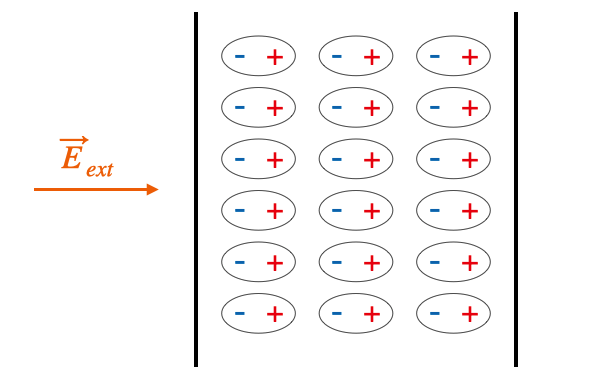
\includegraphics[width=0.6\textwidth]{Electroestática/Dipolos/material_dielectrico.png}
    \caption*{Polarización de los átomos/moléculas del material a causa de un campo $\Vec{E}_{ext}$}
\end{figure}

\subsection{Polarización}

La polarización ($\Vec{P}$) de un material dieléctrico es el momento dipolar por unidad de volumen.

\[d\Vec{p}=\Vec{P}(\Vec{r})d\V\]

Con esto, se puede obtener el potencial de un material polarizado como

\begin{equation}
\begin{split}
    V(\Vec{r}) &= \frac{1}{4\pi\epsilon_o}\int
    \frac{1}{\|\Vec{r}-\Vec{r}'\|^3}(\Vec{r}-\Vec{r}')
    \cdot d\Vec{p}\\
    &= \frac{1}{4\pi\epsilon_o}\int
    \frac{\Vec{P}(\Vec{r}')\cdot(\Vec{r}-\Vec{r}')}{\|\Vec{r}-\Vec{r}'\|^3}\,d\V'\\
    &= \frac{1}{4\pi\epsilon_o}\int\Vec{P}(\Vec{r}')\cdot
    \nabla\left(\frac{1}{\|\Vec{r}-\Vec{r}'\|}\right)\,d\V'\\
    &= \frac{1}{4\pi\epsilon_o}\int\nabla\cdot\left(
    \frac{\Vec{P}(\Vec{r}')}{\|\Vec{r}-\Vec{r}'\|}\right)\,d\V'-\frac{1}{4\pi\epsilon_o}\int
    \frac{\nabla\cdot\Vec{P}(\Vec{r}')}{\|\Vec{r}-\Vec{r}'\|}
    \,d\V'\\
    &= \frac{1}{4\pi\epsilon_o}\oint
    \frac{1}{\|\Vec{r}-\Vec{r}'\|}
    \Vec{P}(\Vec{r}')\cdot d\Vec{S'}-\frac{1}{4\pi\epsilon_o}\int
    \frac{\nabla\cdot\Vec{P}(\Vec{r}')}{\|\Vec{r}-\Vec{r}'\|}
    \,d\V'\\
\end{split}
\nonumber
\end{equation}
\bigbreak
Las últimas integrales se pueden interpretar como potenciales por una carga superficial y una volumétrica. En base a esto, se definen las densidades de carga de polarización:

\begin{equation}
\begin{split}
    &\sigma_p \equiv \Vec{P}(\Vec{r})\cdot\hat{n}\\
    &\rho_p \equiv -\nabla\cdot\Vec{P}(\Vec{r})
\end{split}
\nonumber
\end{equation}
\bigbreak
Con esto, un medio polarizado posee una carga dada por $\sigma_p$ y $\rho_p$. La densidad de carga total al interior del material es

\[\rho_t = \rho_l+\rho_p\]
\bigbreak
donde $\rho_l$ es la densidad de cara libre, la carga ``natural'' del material. La carga total de polarización

\[Q_p=\oint \Vec{P}\cdot d\Vec{S}-\int\nabla\cdot\Vec{P}\,d\V\]
\bigbreak
por teorema de la divergencia es siempre nula.\\

Si $\Vec{P}$ es constante, el potencial se puede calcular como

\[V(\Vec{r})=\frac{1}{\rho_v}\Vec{P}\cdot\Vec{E}_v\]
\bigbreak
donde $\Vec{E}_v$ es un campo eléctrico virtual para una densidad de carga $\rho_v$ uniforme. El vector $\Vec{P}$ se manifiesta sólo dentro del material.

\subsection{Desplazamiento Eléctrico}

Por la primera ecuación de Maxwell se tiene que

\begin{equation}
\begin{split}
    \nabla\cdot\Vec{E} = \frac{\rho_t}{\epsilon_o}
    & \Leftrightarrow \nabla\cdot\Vec{E} = \frac{\rho_l+\rho_p}{\epsilon_o}\\
    &\Leftrightarrow \epsilon\nabla\cdot\Vec{E}=\rho_l -
    \nabla\cdot\Vec{P}\\
    &\Leftrightarrow \epsilon\nabla\cdot\Vec{E}
    +\nabla\cdot\Vec{P}=\rho_l\\
    &\Leftrightarrow\nabla\cdot\left(\epsilon_o
    \Vec{E}+\Vec{P}\right) = \rho_l\\
\end{split}
\nonumber
\end{equation}
\bigbreak
Se define el desplazamiento eléctrico como

\[\Vec{D}=\epsilon_o\Vec{E}+\Vec{P}\]
\bigbreak
Con $\Vec{D}$ se puede definir la primera ecuación de Maxwell en electrostática en medios materiales por

\begin{itemize}
    \item \textbf{Forma diferencial:}
    \[\nabla\cdot\Vec{D}=\rho_l\]
    \item \textbf{Forma integral:}
    \[\oint\Vec{D}\cdot d\Vec{S}=Q_{libre\,encerrada}\]
\end{itemize}

\subsection{Dieléctricos Lineales}

Se llama lineal a un material dieléctrico cuya polarización es proporcional al campo eléctrico, esto es

\[\Vec{P}=\epsilon_o\mathcal{X}_e\Vec{E}\]

A la constante $\mathcal{X}_e$ se le denomina susceptibilidad eléctrica y es característica de cada material.\\

Por la definición de desplazamiento eléctrico se tiene

\begin{equation}
\begin{split}
    \Vec{D} &= \epsilon_o\Vec{E}+\Vec{P}\\
    &= \epsilon_o\Vec{E}+\epsilon_o\mathcal{X}_e\Vec{E}\\
    &= \epsilon_o(1+\mathcal{X}_e)\Vec{E}\\
\end{split}
\nonumber
\end{equation}
\bigbreak
A partir de esto se definen:

\begin{itemize}
    \item \textbf{Permitividad Relativa:}
    \[\epsilon_r=1+\mathcal{X}_e\]
    \item \textbf{Permitividad  Absoluta:}
    \[\epsilon = \epsilon_o\epsilon_r\]
\end{itemize}

Al reemplazar $\Vec{D}=\epsilon\Vec{E}$ en la primera ecuación de Maxwell para materiales se obtiene que

\[\nabla\cdot\Vec{E}=\frac{\rho_l}{\epsilon}\]

\subsubsection{Energía}

La energía de un material dieléctrico lineal se puede calcular como

\[U_e=\frac{1}{2}\int\Vec{E}\cdot\Vec{D}\,d\V\]

integrando sobre todo el espacio.
% Esto tiene sentido y es indicación de una pregunta, pero igual no estoy seguro de si es algo que siempre se cumple. 

% Según yo si, porque si tomas un sistema donde no hay dieléctrico, entonces la permitividad es la del vació y con D=eE, se recupera la ecuación que está en energía potencial electroestática

\subsection{Condiciones de Borde}

Dados dos medios dieléctricos lineales, se llama interfaz a la superficie de contacto entre ambos. El campo eléctrico el materiales se puede descomponer en una parten normal (perpendicular) y otro tangencial (paralela) a la interfaz, estas permiten encontrar las condiciones de borde.

\[\Vec{E}_1 = E_{1n}\hat{n}+E_{1t}\hat{t}\]
\[\Vec{E}_2 = E_{2n}\hat{n}+E_{2t}\hat{t}\]

\subsubsection{Componentes Tangenciales}

Se considera $R$ un camino rectangular infinitesimal (permite ver la interfaz como un plano) cerrado y rectangular, con lados paralelos y perpendiculares a la interfaz que pasa por los dos materiales. La segunda ecuación de Maxwell en electrostática indica que la integral del campo eléctrico en $R$ es nula. Si se hace tender el lado que atraviesa la interfaz a 0, se puede despreciar su contribución a la integral, de modo que


\begin{equation}
\begin{split}
    \oint_R\Vec{E}\cdot d\Vec{l} &= 
    \int_\rightarrow\Vec{E}\cdot d\Vec{l}+
    \int_\uparrow \Vec{E}\cdot d\Vec{l}+
    \int_\leftarrow \Vec{E}\cdot d\Vec{l}+
    \int_\downarrow \Vec{E}\cdot d\Vec{l}\\
    &= \int_\rightarrow\Vec{E}\cdot d\Vec{l}+
    \int_\leftarrow\Vec{E}\cdot d\Vec{l}\\
    &= \int_\rightarrow E_{1t}\,dl+
    \int_\leftarrow E_{2t}\, dl\\
    &= \int_\rightarrow E_{1t}-E_{2t}\, dl\\
    &= 0\\
    &\Rightarrow E_{1t}=E_{2t}\\
\end{split}
\nonumber
\end{equation}
\bigbreak
la componente tangencial del $\Vec{E}$ es continua en la interfaz.

% Puse la imágen para complementar, pero no se si dejarla o no, que opinas? (también creé del desplazamiento)
\begin{figure}[H]
    \centering
    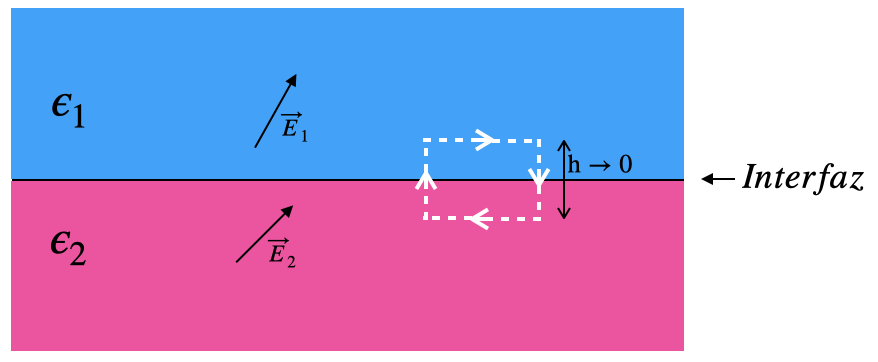
\includegraphics[width=0.5\textwidth]{Electroestática/Dipolos/c_borde_campoe.png}
\end{figure}

\subsubsection{Componentes Normales}

Se considera un cilindro infinitesimal con eje perpendicular a la interfaz y centrado en la misma. Si se hace tender su altura 0, se puede despreciar la superficie del manto y tomar la carga de la interfaz como la única encerrada, de modo que, para $S_1$ la tapa inferior y $S_2$ la tapa superior, por ley de Gauss se tiene que

\begin{equation}
\begin{split}
    \oint\Vec{D}\cdot d\Vec{S}&=\int_{S_1}\Vec{D}\cdot d\Vec{S}+\int_{S_2}\Vec{D}\cdot d\Vec{S}\\
    &=\int_{S_1}D_{1n}\,dS+\int_{S_2}D_{2n}\,dS\\
    &=\int_{S_2}(D_{2n}-D_{1n})\,dS\\
    &=A(D_{2n}-D_{1n})\\
    &=A\sigma_l\\
    &\Rightarrow D_{2n}-D_{1n} = \sigma_l\\
\end{split}
\nonumber
\end{equation}
\bigbreak

donde $A$ es el área de las tapas del cilindro y $\sigma_l$ la densidad de carga de la interfaz.

\begin{figure}[H]
    \centering
    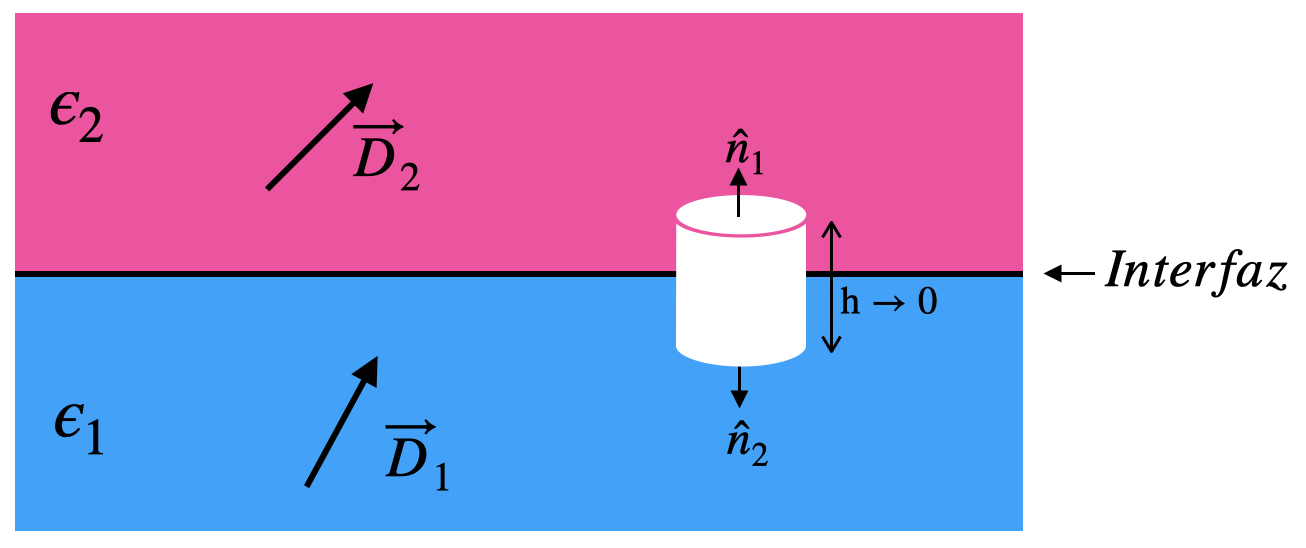
\includegraphics[width=0.5\textwidth]{Electroestática/Dipolos/c_borde_desplaz.png}
\end{figure}

\newpage